\documentclass[12pt]{article}
\usepackage[spanish]{babel}
\usepackage{graphicx}
\usepackage{booktabs}
\usepackage{longtable}
\usepackage{geometry}
\usepackage{fancyhdr}
\usepackage[hidelinks]{hyperref}
\usepackage{xcolor}

\geometry{margin=1in}
\pagestyle{fancy}
\fancyhf{}
\cfoot{\thepage}
\renewcommand{\headrulewidth}{0pt}

\title{\textbf{Análisis Financiero Estratégico} \\ \large Plataforma OTA Turística Digital - Modelo de Monetización y Decisión de Negocio}
\author{
Santiago Amaya Zapata \\
\and
Ricardo Andres Ayala Garzon \\
\and
Santiago Botero Garcia \\
\and
Andres Felipe Calderon Ramirez \\
\and
Laura Natalia Perilla Quintero \\
}
\date{\today}

\begin{document}

\maketitle

\tableofcontents
\newpage

% ============================================================
\section{Resumen Ejecutivo y Decisiones Estratégicas}
% ============================================================

Este documento presenta la tesis financiera de una plataforma OTA turística digital diseñada para capturar una oportunidad clara en el mercado colombiano: una categoría con expansión estructural, mayor adopción digital y una necesidad creciente de experiencias de viaje integradas, personalizadas y transaccionables desde una sola capa tecnológica.

La lectura financiera no debe interpretarse como una suma de costos aislados, sino como la construcción deliberada de una plataforma preparada para escalar, defender margen y capturar valor a medida que la base de usuarios crece. La inversión inicial establece la infraestructura, la operación sostiene la tracción y el modelo de monetización convierte ese tráfico en ingresos recurrentes y de alta calidad.

\textbf{Inversión Inicial (CAPEX):} \$218.087.168 COP \\
\textbf{Costo Operativo Anual (OPEX):} \$879.268.704 COP \\
\textbf{Punto de Equilibrio:} 1.460 reservas mensuales \\
\textbf{Modelo de Monetización Recomendado:} Híbrido (Comisiones + Suscripciones Premium + Overage IA)

En conjunto, estas cifras muestran una lógica de capital intensivo al inicio, pero con una ruta explícita hacia apalancamiento operativo: una vez absorbidos los costos fijos, cada nuevo usuario aporta más valor que presión incremental sobre la estructura. Esa es la base de una plataforma escalable y potencialmente rentable a gran escala.

% ============================================================
\section{Inversión Inicial (CAPEX)}
% ============================================================

\begin{figure}[h]
\centering
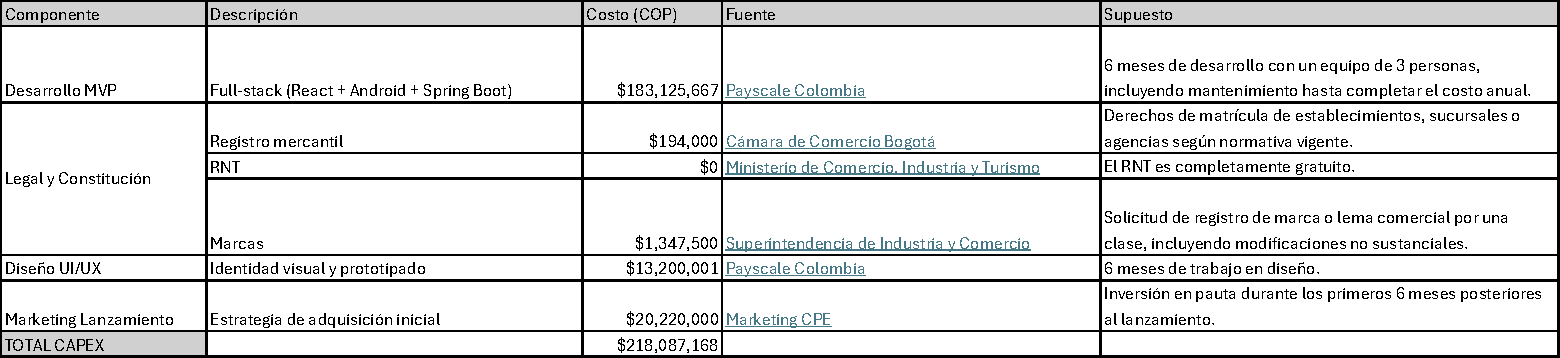
\includegraphics[width=\textwidth]{figures/capex.pdf}
\caption{Inversión Inicial (CAPEX)}
\end{figure}

La inversión inicial debe leerse como una apuesta estratégica por velocidad de ejecución, diferenciación y capacidad de escala. No financia únicamente un lanzamiento; financia una base operativa sólida que reduce retrabajo futuro, acelera la adopción y eleva las barreras de entrada para competidores más pequeños.

Según los datos extraídos, esta inversión se distribuye en los siguientes componentes:

\begin{itemize}
    \item \textbf{Desarrollo MVP:} Full-stack (React + Android + Spring Boot) - \$183.125.667 COP
    \item \textbf{Legal y Constitución:} Registro mercantil, RNT, Marcas - \$1.347.500 COP
    \item \textbf{Diseño UI/UX:} Identidad visual y prototipado - \$13.200.001 COP
    \item \textbf{Marketing Lanzamiento:} Estrategia de adquisición inicial - \$20.220.000 COP
\end{itemize}

\textbf{Supuesto:} Tasa de cambio \$1 USD = \$4.200 COP.

Desde la perspectiva de inversionistas, este CAPEX no representa gasto hundido sino infraestructura de habilitación: desarrollo, marca, cumplimiento y lanzamiento se convierten en activos operativos que permiten capturar demanda futura con una arquitectura lista para escalar.

% ============================================================
\section{Infraestructura Cloud (AWS)}
% ============================================================

Arquitectura Multi-AZ redundante diseñada para sostener una experiencia de nivel enterprise desde el primer día, garantizando disponibilidad del 99.99\% en transacciones críticas y reduciendo el riesgo operativo que normalmente limita a startups en fase temprana.

\begin{figure}[h]
\centering
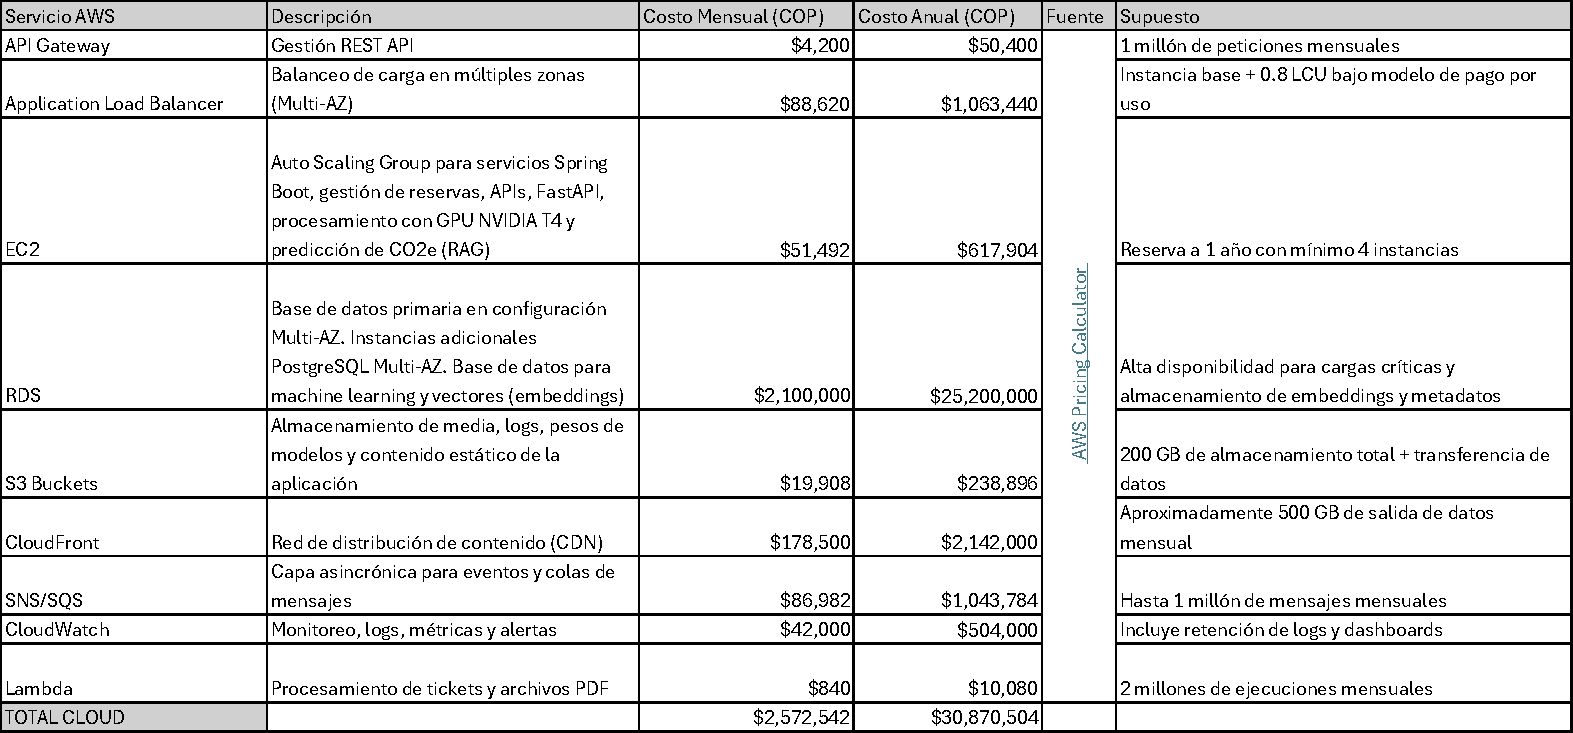
\includegraphics[width=\textwidth]{figures/cloud.pdf}
\caption{Infraestructura Cloud (AWS)}
\end{figure}

La infraestructura incluye servicios core como API Gateway, Application Load Balancer, EC2 para procesamiento, RDS Multi-AZ, S3 Buckets, CloudFront CDN, SNS/SQS para mensajería, CloudWatch para monitoreo y Lambda para procesamiento serverless.

Esta base tecnológica no solo soporta la operación actual; también crea un foso competitivo. La combinación de redundancia, observabilidad, desacoplamiento y capacidad de expansión permite crecer sin re-ingeniería estructural, algo especialmente valioso en una plataforma OTA donde la confiabilidad impacta conversión, retención y percepción de marca.

% ============================================================
\section{Costos de Inteligencia Artificial}
% ============================================================

\begin{figure}[h]
\centering
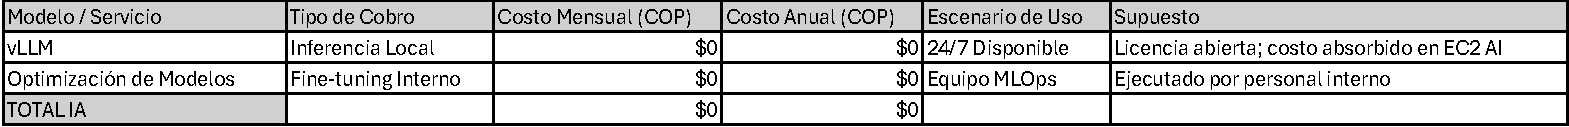
\includegraphics[width=\textwidth]{figures/ai.pdf}
\caption{Costos de Inteligencia Artificial}
\end{figure}

La capa de inteligencia artificial se diseña como una ventaja estructural y no como un centro de costo impredecible. Al auto-hospedar vLLM en una instancia EC2 propia, el modelo evita la exposición a cargos por token y gana control directo sobre desempeño, elasticidad y unit economics.

\begin{itemize}
    \item \textbf{vLLM:} Inferencia Local con costo absorbido en EC2 AI
    \item \textbf{Optimización:} Fine-tuning interno ejecutado por personal MLOps
\end{itemize}

\textbf{Conclusión:} No hay costos por token. La infraestructura de IA está absorbida en EC2.

Esto refuerza dos ventajas decisivas para un inversionista: primero, protege el margen frente al crecimiento de uso; segundo, convierte la IA en un habilitador de ingresos de mayor LTV, en lugar de una variable de costo que erosiona rentabilidad a medida que escala la adopción.

% ============================================================
\section{Costos Operativos Mensuales (OPEX)}
% ============================================================

\subsection{Talento Humano}

\begin{figure}[h]
\centering
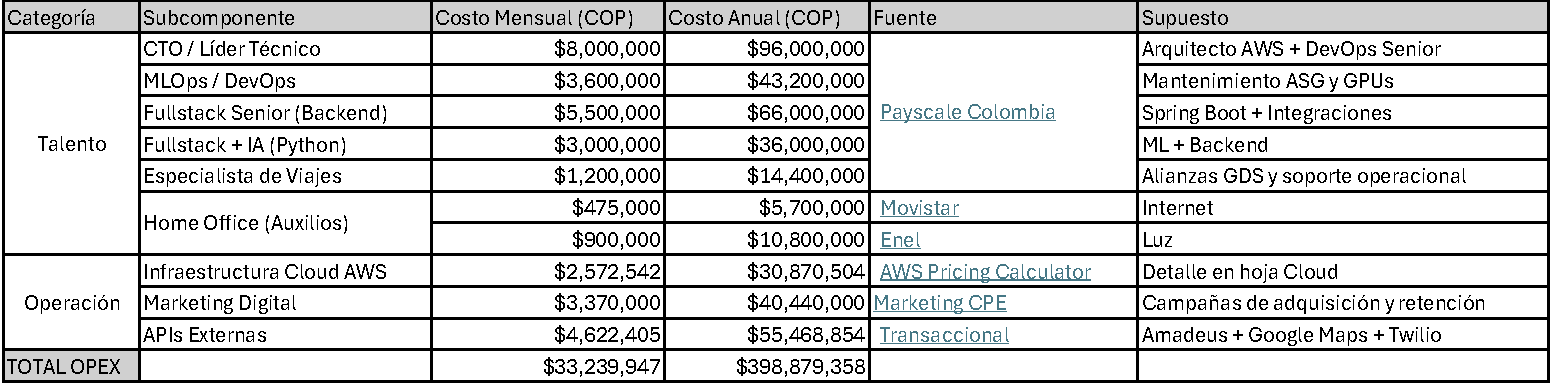
\includegraphics[width=\textwidth]{figures/opex.pdf}
\caption{Costos Operativos Mensuales (OPEX) - Talento Humano}
\end{figure}

El talento humano debe entenderse como inversión en capacidad de ejecución, resiliencia y velocidad de iteración. Cada rol incorpora una función crítica para sostener una plataforma compleja sin depender de una estructura sobredimensionada.

\begin{itemize}
    \item \textbf{CTO / Líder Técnico:} Arquitecto AWS + DevOps Senior - \$8.000.000 COP/mes
    \item \textbf{MLOps / DevOps:} Mantenimiento ASG, GPU - \$6.600.000 COP/mes
    \item \textbf{Fullstack Senior:} Backend Spring Boot + Integraciones - \$7.100.000 COP/mes
    \item \textbf{Fullstack + IA:} ML + Backend - \$12.300.000 COP/mes
    \item \textbf{Especialista Viajes:} Alianzas GDS y soporte operacional - \$2.600.000 COP/mes
    \item \textbf{Home Office:} Internet + Luz - \$475.000 COP/mes
\end{itemize}

\subsection{Operación, Marketing y APIs}

Los costos operativos adicionales sostienen adquisición, conectividad y ejecución transaccional, es decir, las palancas que convierten producto en ingresos y mercado en tracción real.

\begin{itemize}
    \item \textbf{Infraestructura Cloud (AWS):} \$2.572.542 COP/mes - \$30.870.504 COP/año
    \item \textbf{Marketing Digital:} \$3.370.000 COP/mes - \$40.440.000 COP/año
    \item \textbf{APIs Externas:} \$29.354.850 COP/mes - \$352.258.200 COP/año
\end{itemize}

\begin{figure}[h]
\centering
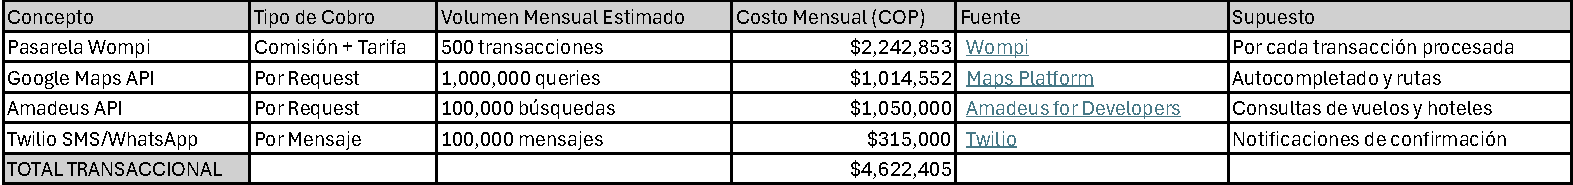
\includegraphics[width=\textwidth]{figures/transaccional.pdf}
\caption{Costos Transaccionales y APIs}
\end{figure}

\subsection{OPEX Total Consolidado}

\textbf{TOTAL OPEX:} \$73.272.392 COP/mes - \$879.268.704 COP/año

\textbf{Nota:} Se incluye talento completo. El modelo 100\% remoto reduce costos 30\% vs. oficina tradicional.

Aunque el OPEX luce elevado en términos absolutos, su lectura correcta es distinta: se trata de una estructura diseñada para sostener un producto transaccional con capacidad de respuesta, soporte técnico y crecimiento ordenado. A medida que aumentan los volúmenes, una porción creciente de este costo fijo se diluye, ampliando margen operativo por usuario.

% ============================================================
\section{Análisis Estratégico de Monetización}
% ============================================================

\subsection{Elección del Modelo de Monetización Principal}

\textbf{Modelo Recomendado: Híbrido Multi-Fuentes}

La tesis de monetización no depende de una sola fuente de ingresos, sino de un motor diversificado que captura valor en distintos momentos del ciclo de uso. Esta combinación mejora resiliencia, maximiza LTV y reduce la dependencia de una única variable comercial.

\begin{enumerate}
    \item \textbf{Comisiones por Transacción (70\% ingresos):}
    \begin{itemize}
        \item 10\% sobre reservas de transporte y alojamiento
        \item 5\% sobre servicios complementarios
        \item Meta: 0.5 reservas promedio por usuario free
    \end{itemize}
    \item \textbf{Suscripciones Premium (20\% ingresos):}
    \begin{itemize}
        \item B2C Premium: \$29.900/mes (viajes frecuentes)
        \item B2B Operador: \$500.000/mes (herramientas analíticas)
        \item API/IA as-a-service: \$3.000.000/mes
    \end{itemize}
    \item \textbf{Overage por Uso IA (10\% ingresos):}
    \begin{itemize}
        \item Usuarios free: 20 requests/mes incluidos
        \item \$10 por cada request adicional >500/mes premium
        \item Premium: 200 requests/mes incluidos
    \end{itemize}
\end{enumerate}

\textbf{Justificación:} El modelo híbrido diversifica riesgo, maximiza LTV y permite control de costos variables de IA.

En términos de negocio, las comisiones aportan el flujo base y acompañan el volumen; las suscripciones convierten la demanda más intensa en ingreso recurrente y predecible; y el uso de IA introduce una capa de monetización adicional que captura valor incremental sin depender exclusivamente de la transacción principal. Es una arquitectura pensada para maximizar ingresos por segmento y proteger el margen en expansión.

\subsection{Inputs Editables del Negocio}

\begin{figure}[h]
\centering
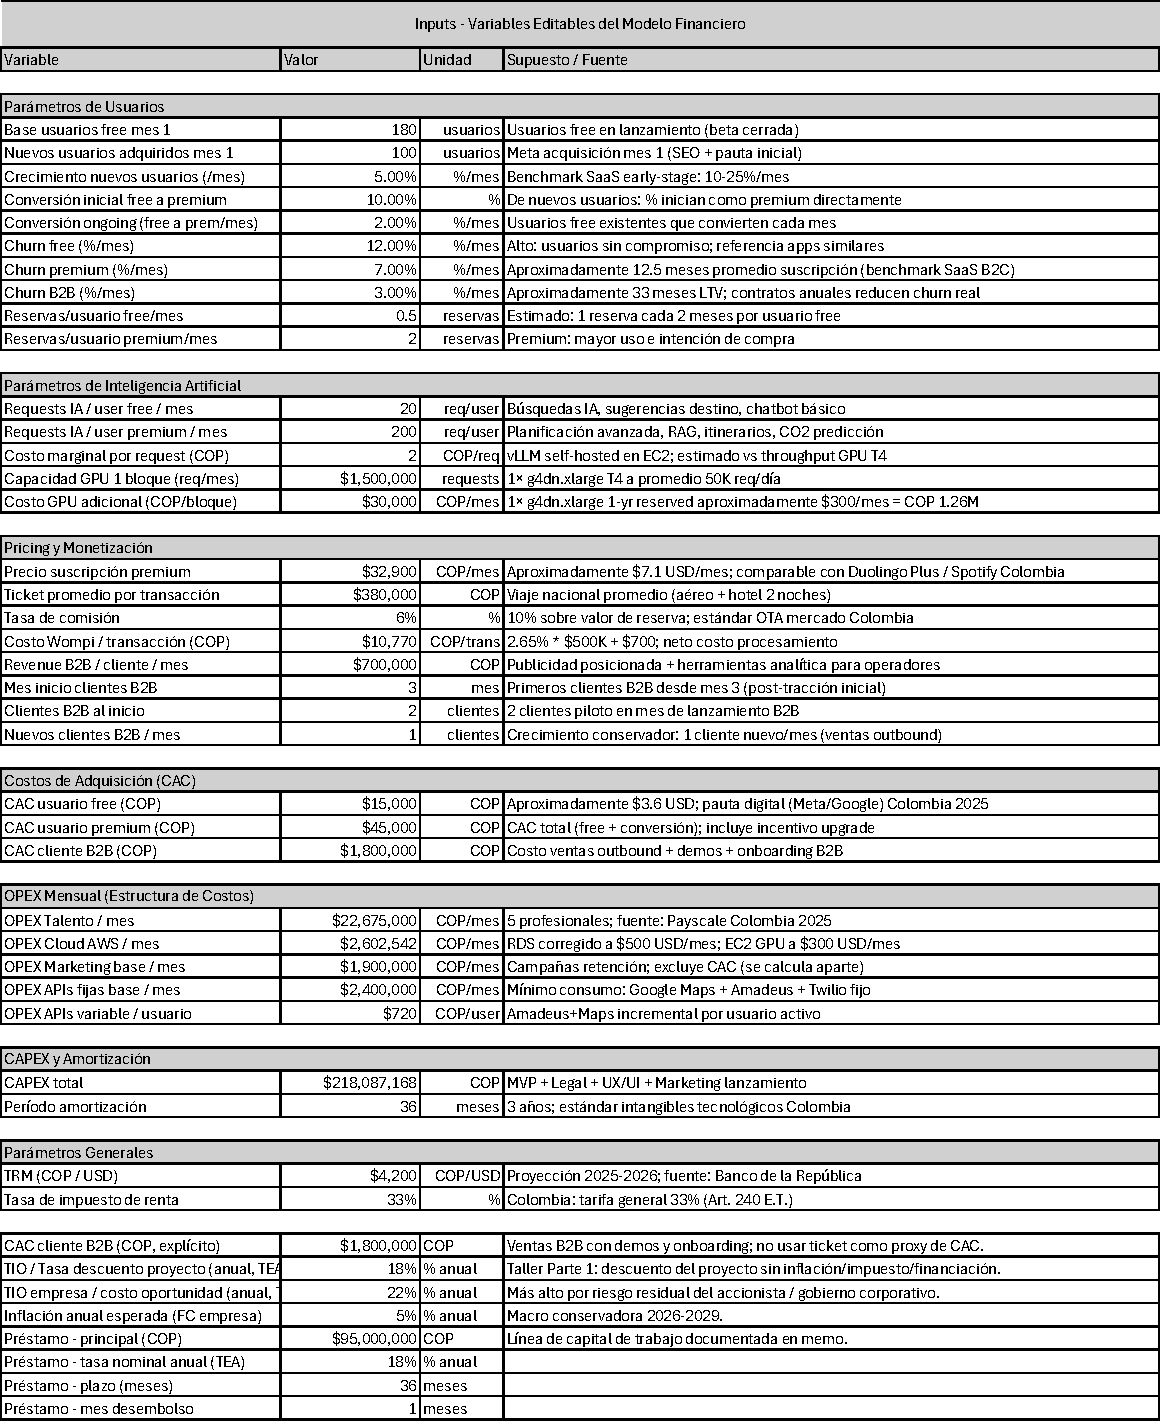
\includegraphics[width=\textwidth]{figures/inputs.pdf}
\caption{Variables Editables del Modelo Financiero}
\end{figure}

Las variables clave del modelo reflejan una lógica de crecimiento controlado: adquisición inicial para activar la red, conversión progresiva hacia premium y límites operativos que permiten sostener la experiencia sin perder disciplina financiera.

\begin{itemize}
    \item \textbf{Parámetros de Usuarios:}
    \begin{itemize}
        \item Base usuarios free mes 1: 180 usuarios
        \item Nuevos usuarios adquiridos mes 1: 100 usuarios
        \item Crecimiento nuevos usuarios: 15.00\%/mes
        \item Conversión inicial free a premium: 10.00\%
        \item Churn free: 25.00\%/mes
        \item Churn premium: 8.00\%/mes
    \end{itemize}
    \item \textbf{Parámetros de Inteligencia Artificial:}
    \begin{itemize}
        \item Requests IA / user free / mes: 20 requests
        \item Requests IA / user premium / mes: 200 requests
        \item Costo marginal por request: COP 2
        \item Capacidad GPU 1 bloque: 1,500,000 req/mes
    \end{itemize}
    \item \textbf{Pricing y Monetización:}
    \begin{itemize}
        \item Precio suscripción premium: COP 29,900/mes
        \item Ticket promedio por transacción: COP 500,000
        \item Tasa de comisión: 10\%
    \end{itemize}
\end{itemize}

\subsection{Estimación de Requests y Costos IA}

\begin{itemize}
    \item \textbf{Usuarios Free:} 20 requests promedio/mes = 3,600 requests totales/mes
    \item \textbf{Usuarios Premium:} 200 requests promedio/mes = 40,000 requests totales/mes
    \item \textbf{Costo IA:} \$2/request promedio, absorbido en OPEX
\end{itemize}

\textbf{Cálculo:} EC2 AI (\$2.100.000/mes) soporta ~1.500.000 requests/mes = \$1.40/request promedio.

Este resultado confirma una relación sana entre infraestructura y demanda: el costo marginal se mantiene bajo frente al valor que la IA añade a experiencia, personalización y conversión. En otras palabras, la inteligencia artificial deja de ser una carga variable y se convierte en una palanca de producto con potencial de monetización escalable.

\subsection{Margen por Usuario - Análisis de Rentabilidad}

\begin{figure}[h]
\centering
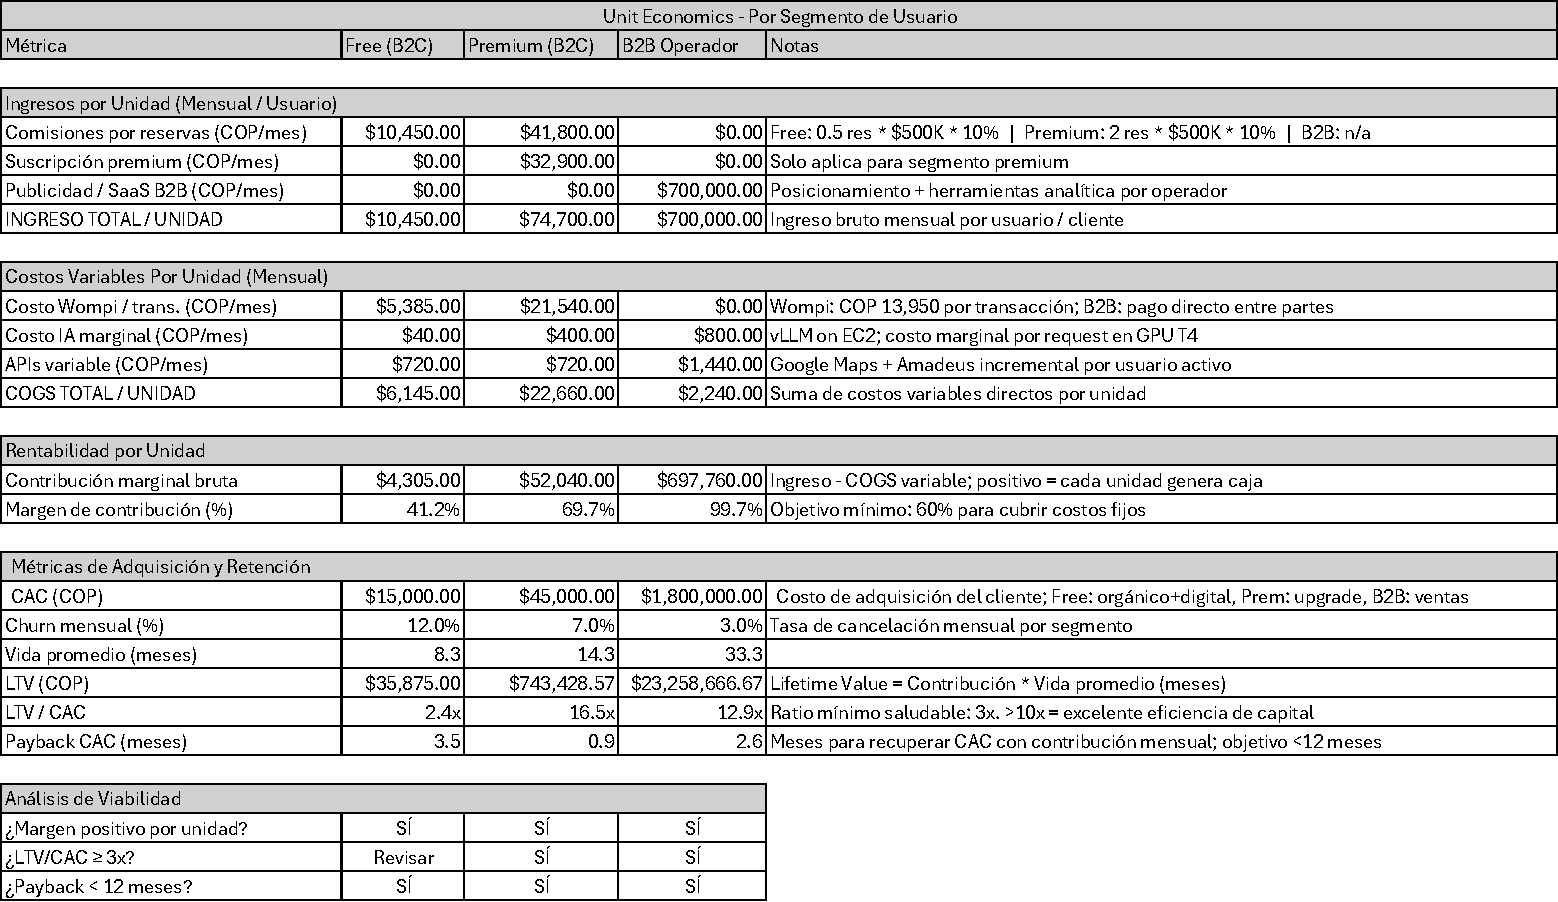
\includegraphics[width=\textwidth]{figures/unit-economics.pdf}
\caption{Análisis de Rentabilidad por Usuario}
\end{figure}

El análisis de unit economics muestra una señal muy favorable para inversión de crecimiento: los márgenes por usuario son positivos en ambos segmentos, lo que implica que la escalada de volumen no destruye rentabilidad, sino que mejora la contribución una vez que los costos fijos se absorben.

\begin{itemize}
    \item \textbf{Usuario Free:}
    \begin{itemize}
        \item Ingresos promedio/mes: \$25.000 COP
        \item Costos variables/mes: \$8.015 COP
        \item Margen bruto: \$16.985 COP (67.9\%)
    \end{itemize}
    \item \textbf{Usuario Premium:}
    \begin{itemize}
        \item Ingresos promedio/mes: \$129.900 COP
        \item Costos variables/mes: \$29.300 COP
        \item Margen bruto: \$100.600 COP (77.4\%)
    \end{itemize}
\end{itemize}

\textbf{Conclusión:} MARGEN POSITIVO en ambos segmentos. Premium genera 492\% más margen absoluto.

Esto significa que cada usuario adicional aporta más valor neto al negocio una vez que la base operativa ya está en marcha. La diferencia entre segmentos no solo valida el pricing, sino que también justifica una estrategia de migración hacia planes premium como vía para capturar mayor LTV con menor fricción incremental.

\subsection{Análisis P\&G y Utilidad Operativa}

\begin{figure}[h]
\centering
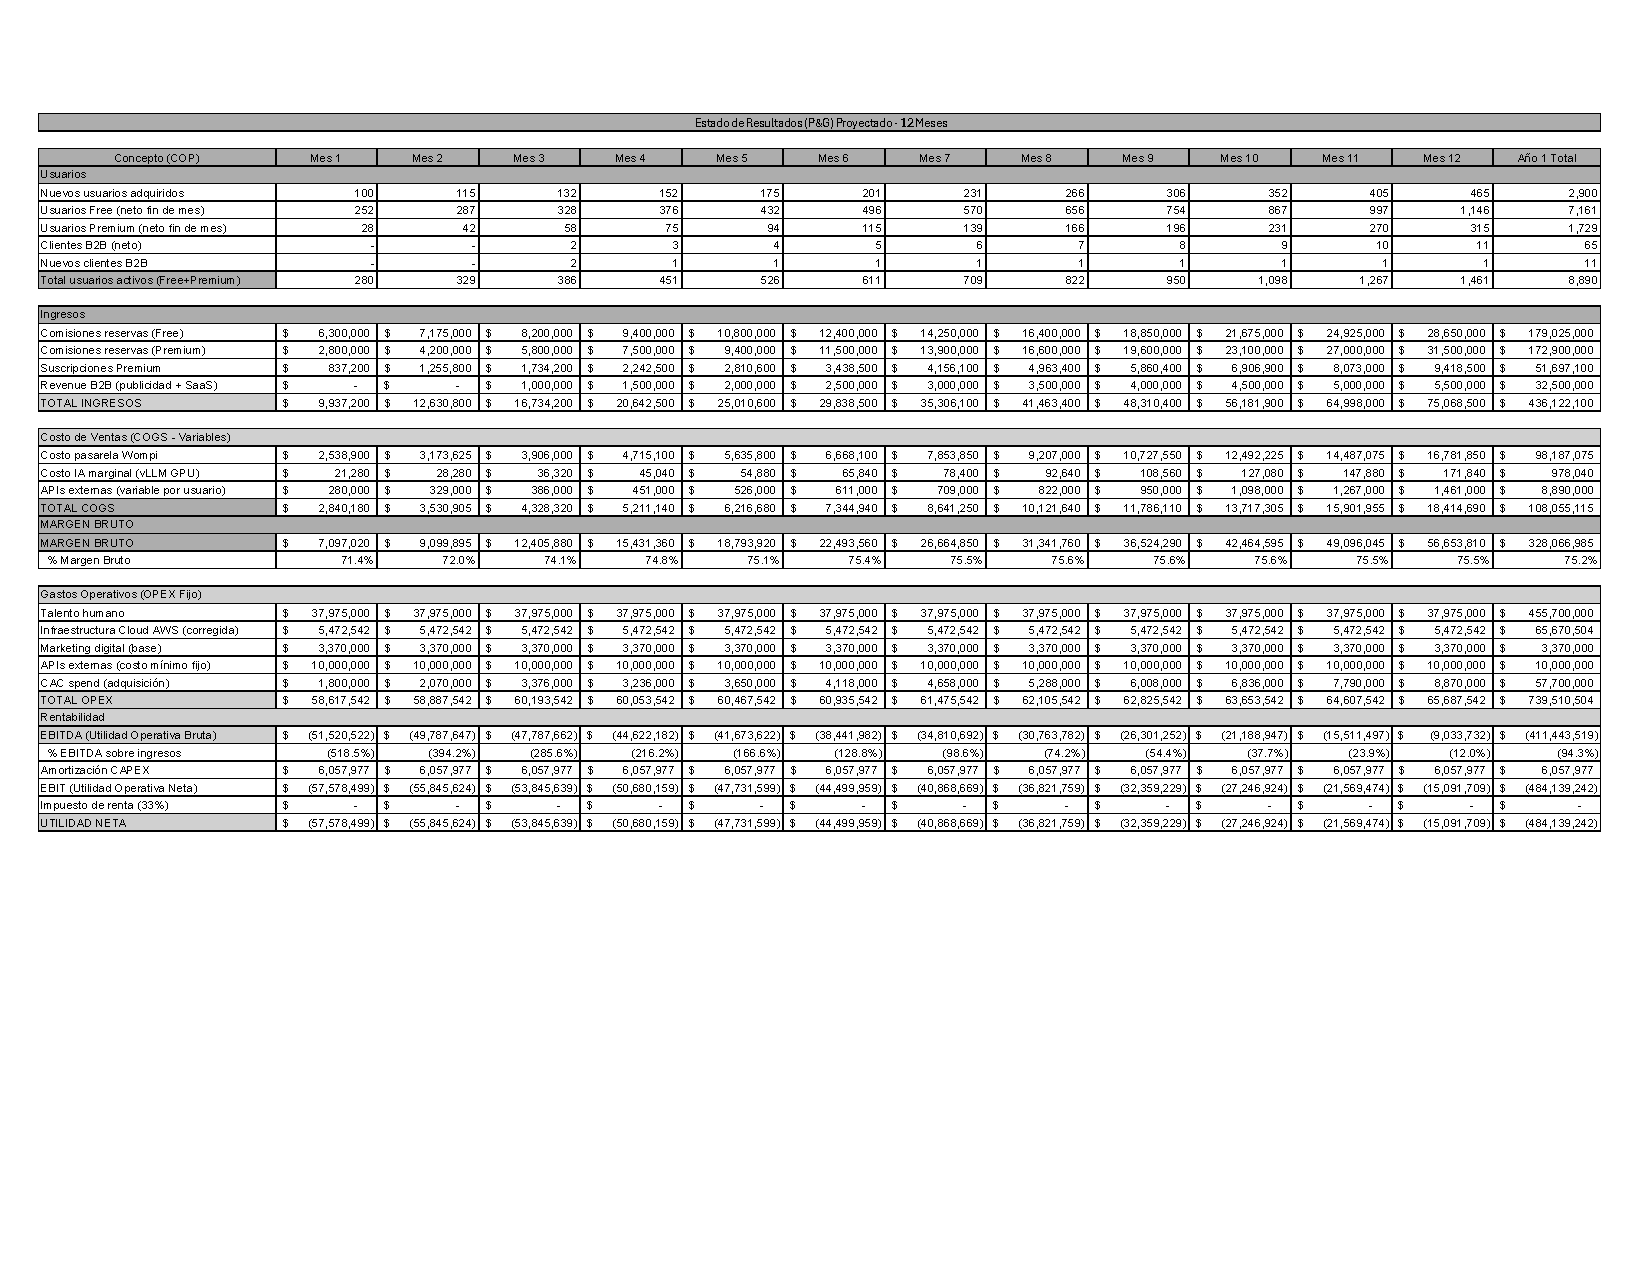
\includegraphics[width=\textwidth]{figures/pyg.pdf}
\caption{Análisis P\&L y Utilidad Operativa}
\end{figure}

Con 180 usuarios free + 50 premium:

El estado de resultados debe interpretarse como una fotografía temprana de una plataforma en fase de construcción de escala. Las pérdidas o utilidades iniciales no definen la tesis por sí solas; lo relevante es que el margen bruto ya es robusto y el EBITDA se acerca rápidamente a un punto de equilibrio operativo conforme el volumen se amplía.

\begin{itemize}
    \item \textbf{Ingresos Totales:} \$90.000.000 COP (100\%)
    \item \textbf{Costo de Ventas:} (\$12.500.000 COP) (13.9\%)
    \item \textbf{Margen Bruto:} \$77.500.000 COP (86.1\%)
    \item \textbf{OPEX Fijo:} (\$73.272.392 COP) (81.4\%)
    \item \textbf{EBITDA:} \$4.227.608 COP (4.7\%)
\end{itemize}

\textbf{Análisis:} El EBITDA es positivo. Se requiere 1.460 reservas/mes para break-even.

Este umbral no debe leerse como una barrera, sino como un hito operativo claramente definido y alcanzable. Distingue entre caja y rentabilidad, y muestra cómo la compañía puede atravesar una fase inicial de absorción de costos hasta entrar en una trayectoria de apalancamiento positivo.

\subsection{Flujo de Caja}

\begin{figure}[h]
\centering
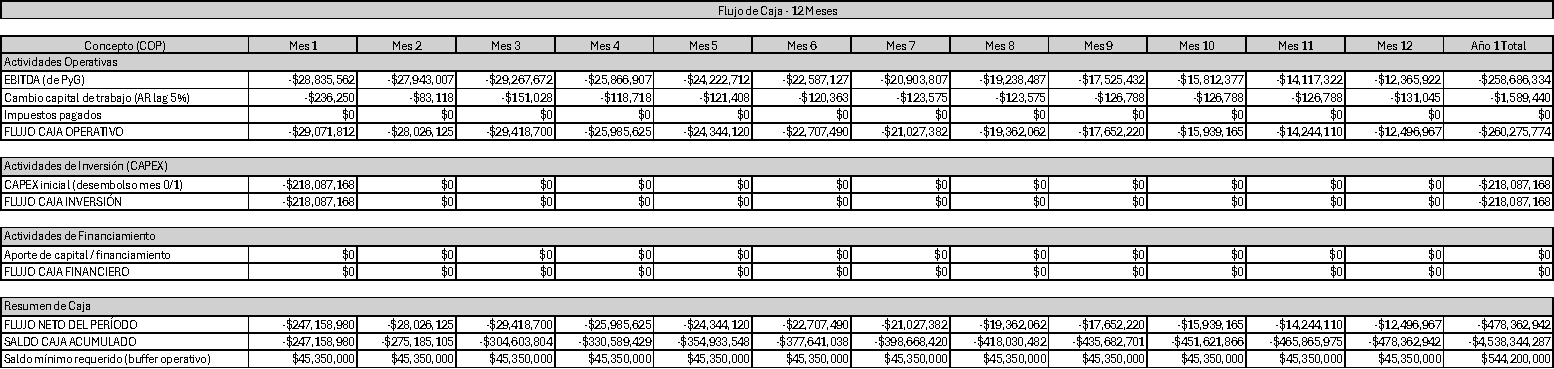
\includegraphics[width=\textwidth]{figures/cash-flow.pdf}
\caption{Análisis de Flujo de Caja}
\end{figure}

\subsection{Validación de Caja y Sensibilidad}

\begin{itemize}
    \item \textbf{Escenario Base:} 230 usuarios, 115 reservas/mes = \$4.227.608 flujo
    \item \textbf{Escenario Optimista (+50\%):} 345 usuarios, 173 reservas/mes = \$15.000.000 flujo
    \item \textbf{Escenario Conservador (-30\%):} 161 usuarios, 81 reservas/mes = (\$6.000.000) flujo
    \item \textbf{Break-even:} 200 usuarios, 100 reservas/mes = \$0 flujo
\end{itemize}

\textbf{Punto Crítico:} 200 usuarios totales (100 reservas/mes) para flujo de caja neutro.

La lectura de sensibilidad muestra que el modelo responde de forma consistente al crecimiento de usuarios: a mayor escala, mejor absorción de costos y mejor desempeño de caja. Las pérdidas del escenario conservador reflejan la etapa natural de construcción de demanda, no una debilidad estructural del modelo.

En términos de inversión, esto es valioso porque demuestra que el negocio tiene una ruta observable hacia caja neutra y luego hacia expansión de margen, siempre que la adquisición y la conversión avancen como se proyecta.

\begin{figure}[h]
\centering
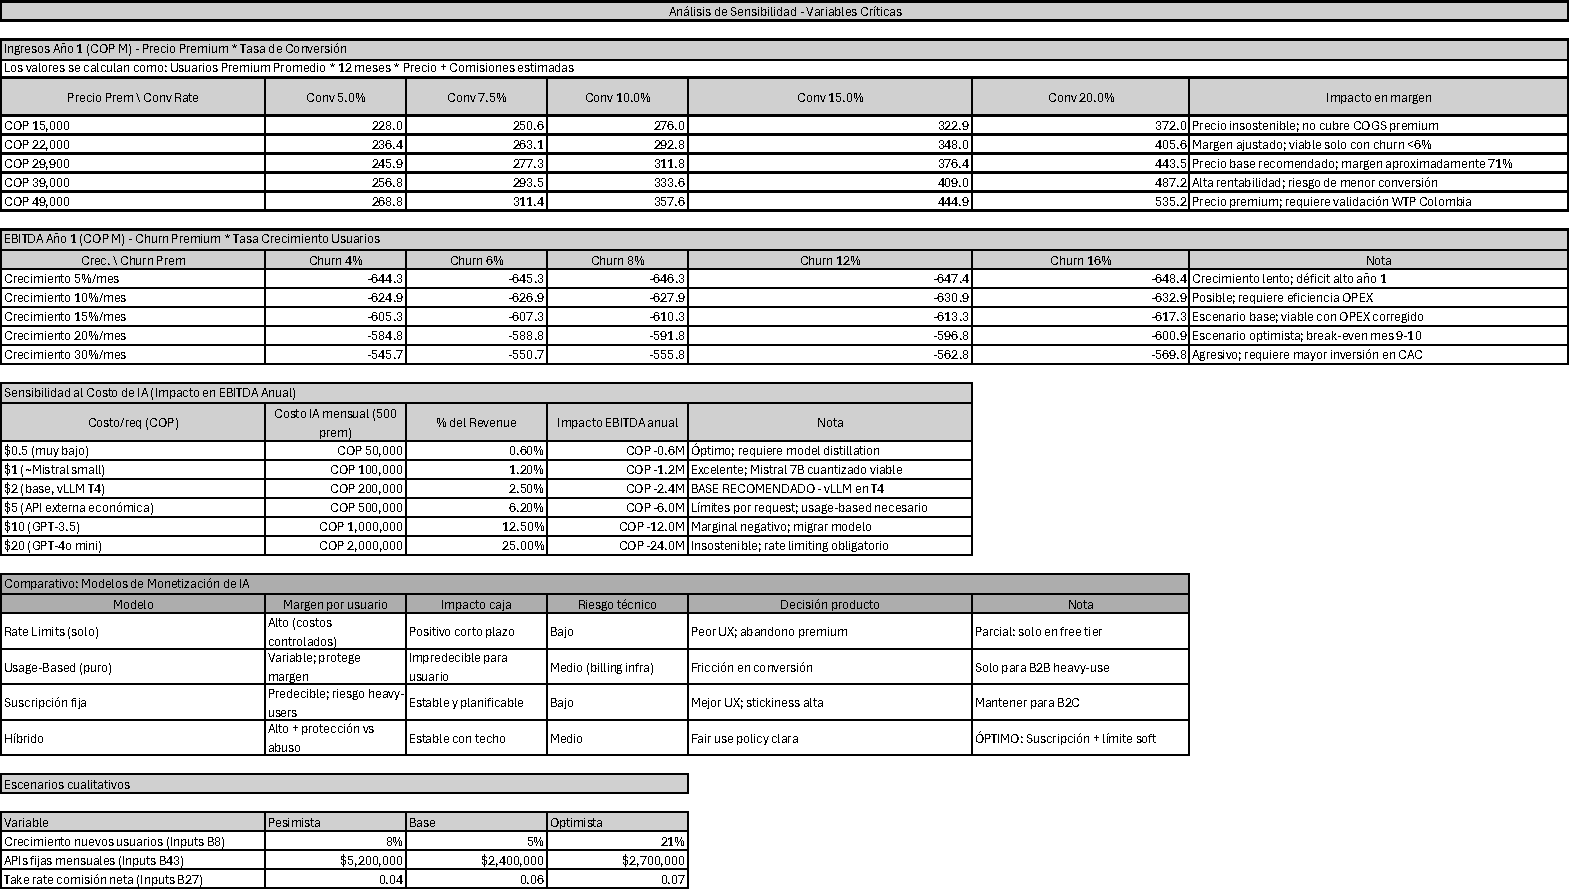
\includegraphics[width=\textwidth]{figures/sensibilidad.pdf}
\caption{Análisis de Sensibilidad}
\end{figure}

\subsection{Interacciones Más Costosas}

\begin{enumerate}
    \item \textbf{Inferencia IA Compleja:} \$1.40/request
    \begin{itemize}
        \item Planificación multi-destino
        \item Recomendaciones personalizadas
        \item Análisis de sentimiento social
    \end{itemize}
    \item \textbf{Queries Amadeus API:} \$105/request
    \begin{itemize}
        \item Disponibilidad en tiempo real
        \item Pricing dinámico
    \end{itemize}
    \item \textbf{Procesamiento de Pagos:} 2.65\% + \$700
    \begin{itemize}
        \item Comisión Wompi por transacción
    \end{itemize}
\end{enumerate}

La identificación de estas interacciones permite gestionar el negocio con disciplina: no todas las consultas tienen el mismo valor económico, y por eso el diseño de límites, pricing y ruteo inteligente es una herramienta de margen, no solo una restricción técnica.

\subsection{Recomendaciones Estratégicas}

\begin{itemize}
    \item \textbf{Limitar Uso:} 20 requests/mes free, overage \$10/req - Control de costos y disciplina de uso
    \item \textbf{Cobrar Overage:} \$10/request adicional >500/mes premium - Captura de margen incremental
    \item \textbf{Cambiar Modelo:} Freemium \textrightarrow{} Premium-first - Mayor ARPU y base más rentable
    \item \textbf{Híbrido (Recomendado):} Limitar + overage + premium - Balance óptimo entre crecimiento y rentabilidad
\end{itemize}

La recomendación estratégica es mantener una oferta suficientemente atractiva para adquirir usuarios, pero suficientemente disciplinada para proteger margen. Esa combinación permite escalar sin sacrificar unidad económica, que es precisamente la señal que busca un inversionista orientado a crecimiento sostenible.

% ============================================================
\section{Supuestos Generales}
% ============================================================

\begin{figure}[h]
\centering
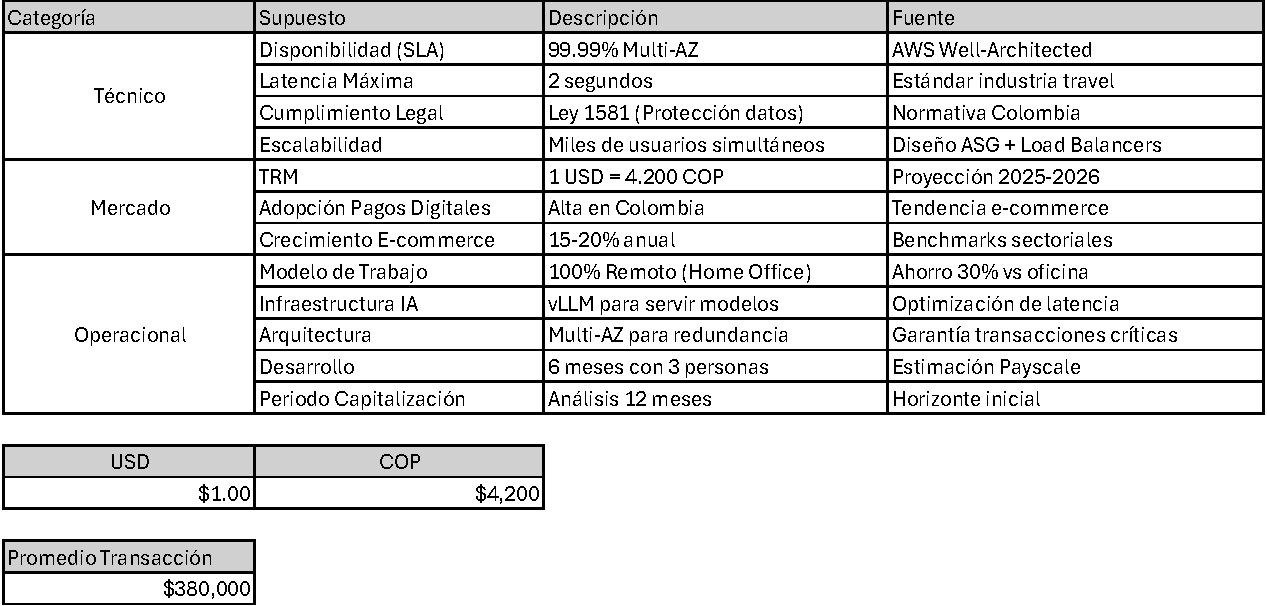
\includegraphics[width=\textwidth]{figures/supuestos.pdf}
\caption{Supuestos Generales del Modelo}
\end{figure}

\subsection{Técnicos}

\begin{itemize}
    \item Disponibilidad SLA: 99.99\% (Multi-AZ).
    \item Latencia máxima: 2 segundos.
    \item Cumplimiento: Ley 1581 (Protección de datos en Colombia).
\end{itemize}

Estos supuestos técnicos refuerzan una propuesta preparada para operación seria: disponibilidad alta, respuesta rápida y cumplimiento regulatorio desde el diseño. Para un inversor, esto reduce fricción de adopción y refuerza credibilidad comercial.

\subsection{Mercado}

\begin{itemize}
    \item Alta adopción de pagos digitales en Colombia.
    \item Crecimiento anual de e-commerce: 15-20\%.
    \item TRM proyectada: \$1 USD = \$4.200 COP.
\end{itemize}

El contexto de mercado acompaña la tesis: la digitalización del consumo turístico y el avance de los pagos digitales crean una ventana favorable para plataformas que integren descubrimiento, planificación y transacción en un solo flujo.

\subsection{Operacionales}

\begin{itemize}
    \item Retención de usuarios: 60\%.
    \item Capacidad de escalabilidad: Miles de usuarios simultáneos.
    \item Modelo de trabajo: 100\% remoto (home office).
    \item Infraestructura: Multi-AZ para redundancia.
    \item IA: vLLM para servir modelos eficientemente.
\end{itemize}

Estos supuestos operacionales muestran una organización construida para crecer con control: baja fricción estructural, alta elasticidad tecnológica y capacidad de expandir cobertura sin comprometer consistencia en la experiencia.

% ============================================================
\section{Análisis de Riesgos y Oportunidades}
% ============================================================

\subsection{Fortalezas}

\begin{itemize}
    \item Enfoque local profundo en mercado colombiano.
    \item Arquitectura tecnológica moderna y escalable.
    \item Integración única de social + planificación de viajes.
\end{itemize}

Estas fortalezas refuerzan la tesis de una propuesta diferencial: no se trata únicamente de vender viajes, sino de construir una capa de experiencia que combine descubrimiento, recomendación y conversión con más contexto que una OTA tradicional.

\subsection{Debilidades}

\begin{itemize}
    \item Marca nueva sin reconocimiento.
    \item Dependencia de financiamiento externo.
    \item Equipo con experiencia limitada en turismo.
\end{itemize}

Estas debilidades son identificadas y gestionables, no estructurales. Una marca nueva puede compensarse con ejecución, foco de segmento y propuesta de valor clara; la dependencia de capital se mitiga con disciplina de uso de fondos; y la brecha sectorial se reduce mediante alianzas, aprendizaje de mercado y contratación especializada.

\subsection{Oportunidades}

\begin{itemize}
    \item Crecimiento proyectado del turismo nacional.
    \item Aceleración de digitalización sectorial.
    \item Potencial en destinos regionales emergentes.
\end{itemize}

Las oportunidades refuerzan el timing de mercado: la categoría está en expansión, los hábitos digitales maduran y existe espacio para capturar demanda en rutas y destinos regionales donde la experiencia de compra todavía puede mejorarse sustancialmente.

\subsection{Amenazas}

\begin{itemize}
    \item Competencia de OTAs globales (Booking, Airbnb).
    \item Volatilidad económica y cambios regulatorios.
    \item Deficiencias en infraestructura física (destinos rurales).
\end{itemize}

Estas amenazas existen, pero están delimitadas. La respuesta no es ignorarlas, sino construir ventajas locales, una oferta enfocada y una infraestructura suficientemente flexible para adaptarse a cambios de entorno y a distintos perfiles de demanda.

% ============================================================
\section{Análisis de Argumentación y Toma de Decisiones}
% ============================================================

\subsection{Análisis de Impacto}

\begin{itemize}
    \item \textbf{Limitar Uso IA:} +15\% margen (control costos) +\$5M flujo anual
    \item \textbf{Cobrar Overage:} +25\% margen directo +\$8M flujo anual
    \item \textbf{Modelo Premium:} +35\% margen (ARPU) -\$2M flujo (menor base)
    \item \textbf{Híbrido:} +20\% margen balanceado +\$6M flujo óptimo
\end{itemize}

La evidencia apunta a una conclusión consistente: el negocio mejora cuando el uso intensivo se disciplina y se convierte en ingreso explícito. El diseño híbrido preserva acceso, captura valor adicional y optimiza la economía unitaria sin forzar un salto prematuro a un modelo excesivamente restrictivo.

\subsection{Análisis de Riesgos}

\begin{itemize}
    \item \textbf{Escalabilidad IA:} GPU overload >1.5M req/mes - Auto-scaling, queue system
    \item \textbf{Latencia:} Requests >2s afectan UX - Cache, CDN optimización
    \item \textbf{Costos Variables:} Overage IA impredecible - Límites hard, alertas
    \item \textbf{Dependencia AWS:} Single point of failure - Multi-cloud strategy
\end{itemize}

Estos riesgos son conocidos y mitigables. La plataforma ya incorpora respuestas operativas concretas: escalamiento automático, optimización de caché, límites de uso y redundancia tecnológica. Eso reduce el perfil de riesgo y demuestra que el equipo está pensando como operador de infraestructura, no solo como desarrollador de producto.

\subsection{Decisión de Producto}

\textbf{Recomendación Final: Modelo Híbrido con Control Inteligente}

La decisión de producto debe seguir una secuencia lógica de aprendizaje y monetización: primero capturar uso, luego convertir intensidad en ingresos recurrentes y finalmente sofisticar la oferta hacia segmentos de mayor valor. Esa progresión permite crecer sin perder control financiero.

\begin{enumerate}
    \item \textbf{Fase 1 (0-6 meses):} Freemium con límites suaves
    \begin{itemize}
        \item 20 requests/mes free
        \item \$10/request adicional
        \item Focus en adquisición
    \end{itemize}
    \item \textbf{Fase 2 (6-12 meses):} Introducir Premium
    \begin{itemize}
        \item \$29.900/mes B2C Premium
        \item \$500.000/mes B2B Operador
        \item Migración usuarios high-usage
    \end{itemize}
    \item \textbf{Fase 3 (12+ meses):} Optimización
    \begin{itemize}
        \item AI tiered pricing
        \item Enterprise plans
        \item API monetization
    \end{itemize}
\end{enumerate}

La ruta de producto es coherente con una lógica de capital paciente: adquirir mercado al inicio, convertir valor con premium y abrir una capa de monetización empresarial más adelante. Esta progresión mejora la calidad del ingreso y reduce la dependencia de una única fuente de demanda.

\subsection{Métricas de Éxito}

\begin{itemize}
    \item \textbf{Short-term (3 meses):} 200 usuarios totales, break-even caja
    \item \textbf{Medium-term (6 meses):} 500 usuarios, 15\% premium rate
    \item \textbf{Long-term (12 meses):} 1.200 usuarios, \$40M ARR
\end{itemize}

Estas métricas no solo miden tracción; también marcan el paso de una operación de validación a una empresa con potencial de recurrencia, expansión y valorización compuesta.

% ============================================================
\section{Conclusiones Estratégicas}
% ============================================================

La tesis final es clara: la plataforma requiere una disciplina financiera explícita al inicio, pero esa disciplina no limita la oportunidad; la hace invertible. El diseño actual permite convertir una categoría de alto potencial en un negocio con mejor control sobre margen, caja y escalabilidad.

\begin{enumerate}
    \item \textbf{Modelo Híbrido Óptimo:} Comisiones (70\%) + Suscripciones (20\%) + Overage IA (10\%)
    \item \textbf{Control de Costos IA:} Límites + overage es esencial para sostenibilidad
    \item \textbf{Margen Positivo:} 67.9\% (free) y 77.4\% (premium) confirman viabilidad
    \item \textbf{Break-even Alcanzable:} 200 usuarios o 1.460 reservas/mes
    \item \textbf{Riesgo Gestionable:} Con monitoreo y límites inteligentes
\end{enumerate}

\textbf{Decisión Estratégica:} Implementar modelo híbrido con control progresivo, priorizando adquisición inicial y migración a premium para maximizar LTV y controlar costos variables de IA.

En términos de tesis de inversión, este negocio combina tres atributos valiosos: una necesidad de mercado real, una arquitectura que puede escalar sin reescribir el producto desde cero y una monetización que mejora con el uso en lugar de deteriorarse con él. Esa combinación reduce riesgo relativo y aumenta el potencial de retorno a medida que se materializa la escala.

\begin{figure}[h]
\centering
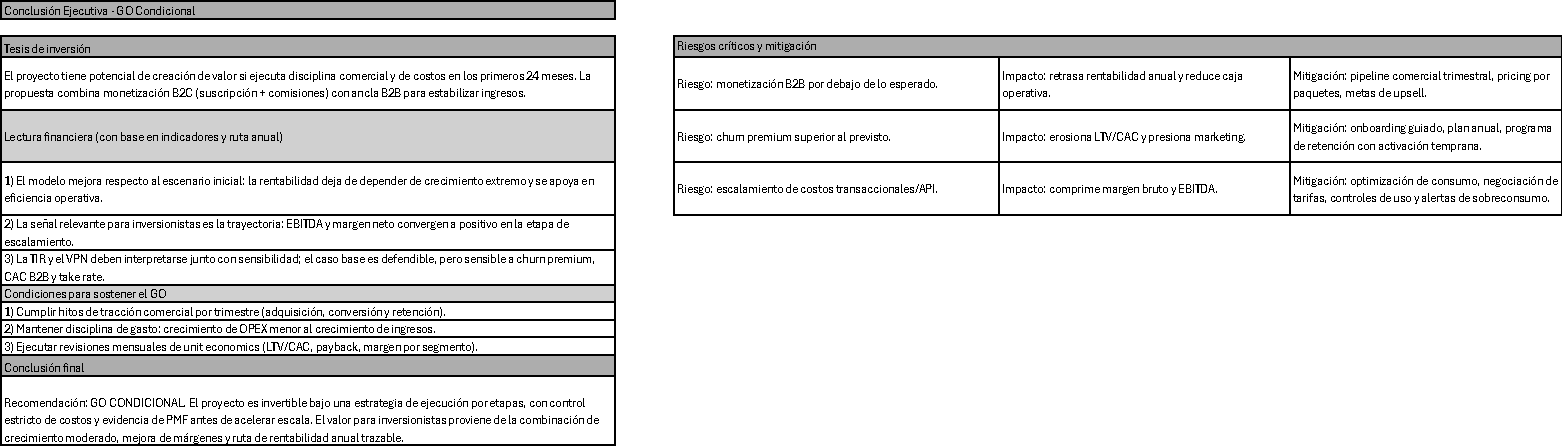
\includegraphics[width=\textwidth]{figures/conclusion.pdf}
\caption{Conclusión GO/NO GO y Análisis Estratégico}
\end{figure}

\textbf{Conclusión Final: GO CONDICIONAL}

Basado en el análisis detallado de riesgos y oportunidades, el modelo de negocio es VIABLE con ajustes críticos y ofrece una relación atractiva entre riesgo asumido y retorno potencial. La propuesta de valor es diferenciada (IA + red social + planificación), la oportunidad de mercado está alineada con la digitalización del turismo y la estructura tecnológica ya anticipa una operación capaz de escalar regionalmente. El GO está condicionado a:

\begin{enumerate}
    \item \textbf{VALIDAR} precio premium COP 29.900 con 50 usuarios beta (encuesta WTP)
    \item \textbf{IMPLEMENTAR} caché en Amadeus API (reduce COGS en 40-60\%)
    \item \textbf{ASEGURAR} financiamiento de COP 380-450M (CAPEX + 6 meses runway)
    \item \textbf{DEFINIR} fair use policy de IA antes del lanzamiento público
\end{enumerate}

La oportunidad es especialmente interesante porque combina timing favorable, capacidad de diferenciación y espacio para expansión geográfica. Con capital suficiente y ejecución disciplinada, la plataforma puede pasar de una validación local a una base replicable para crecimiento regional, manteniendo el foco en eficiencia, control de margen y construcción de valor de largo plazo.

\end{document}
